% !TeX program = lualatex
% !TeX encoding = utf8
% !TeX spellcheck = uk_UA
% !TeX root =../LabWork.tex

%------------- Externalize ------------
%\usetikzlibrary{external}
%\tikzexternalize[prefix=\currfiledir/pictures/]
%\tcbsetforeverylayer{shield externalize}
%--------------------------------------

\def\eff{e\kern-.3ex f\kern-.5ex f}

% -------------------------------------- Grid -------------------------------------------------------
\makeatletter
\def\grd@save@target#1{%
  \def\grd@target{#1}}
\def\grd@save@start#1{%
  \def\grd@start{#1}}
\tikzset{
  grid with coordinates/.style={
    to path={%
      \pgfextra{%
        \edef\grd@@target{(\tikztotarget)}%
        \tikz@scan@one@point\grd@save@target\grd@@target\relax
        \edef\grd@@start{(\tikztostart)}%
        \tikz@scan@one@point\grd@save@start\grd@@start\relax
        \draw[minor help lines] (\tikztostart) grid (\tikztotarget);
        \draw[major help lines] (\tikztostart) grid (\tikztotarget);
        \grd@start
        \pgfmathsetmacro{\grd@xa}{\the\pgf@x/1cm}
        \pgfmathsetmacro{\grd@ya}{\the\pgf@y/1cm}
        \grd@target
        \pgfmathsetmacro{\grd@xb}{\the\pgf@x/1cm}
        \pgfmathsetmacro{\grd@yb}{\the\pgf@y/1cm}
        \pgfmathsetmacro{\grd@xc}{\grd@xa + \pgfkeysvalueof{/tikz/grid with coordinates/major step}}
        \pgfmathsetmacro{\grd@yc}{\grd@ya + \pgfkeysvalueof{/tikz/grid with coordinates/major step}}
        \foreach \x in {\grd@xa,\grd@xc,...,\grd@xb}
        \node[anchor=north] at (\x,\grd@ya) {\pgfmathprintnumber{\x}};
        \foreach \y in {\grd@ya,\grd@yc,...,\grd@yb}
        \node[anchor=east] at (\grd@xa,\y) {\pgfmathprintnumber{\y}};
      }
    }
  },
  minor help lines/.style={
    help lines,
    step=\pgfkeysvalueof{/tikz/grid with coordinates/minor step}
  },
  major help lines/.style={
    help lines,
    line width= 1pt,
    step=\pgfkeysvalueof{/tikz/grid with coordinates/major step}
  },
  grid with coordinates/.cd,
  minor step/.initial=.2,
  major step/.initial=1,
  major line width/.initial=2pt,
}
\makeatother
%============================================= Заголовок документу ====================================================%

\keywords{Змінний струм, $RLC$-коло, активний опір, реактивний опір, ємнісний опір, індуктивний опір, імпеданс, резонанс напруг, резонанс струмів.}
\abstract{Дослідження залежності напруги та сили струму на елементах паралельного та послідовного коливальних контурів. Визначення добротності коливального контуру при різних параметрах контуру.}
\apparatus{генератор сигналів низькочастотний ГЗ-56/1, вольтметр універсальний В7-16А, осцилограф C1-83.}
\chapter{Резонансні явища в колах змінного струму}
\makeworktitle

\section{Обладнання}

\subsection*{Генератор сигналів низькочастотний ГЗ-56/1}

\begin{figure}[h!]
\centering
\begin{tikzpicture}[every pin/.style={minimum size = 5pt, pin edge={red, thick}, draw, fill=gray!5, red, circle, font=\scriptsize},
    small dot/.style={fill=black,circle,scale=0.3}]
    \node at (0,0){ 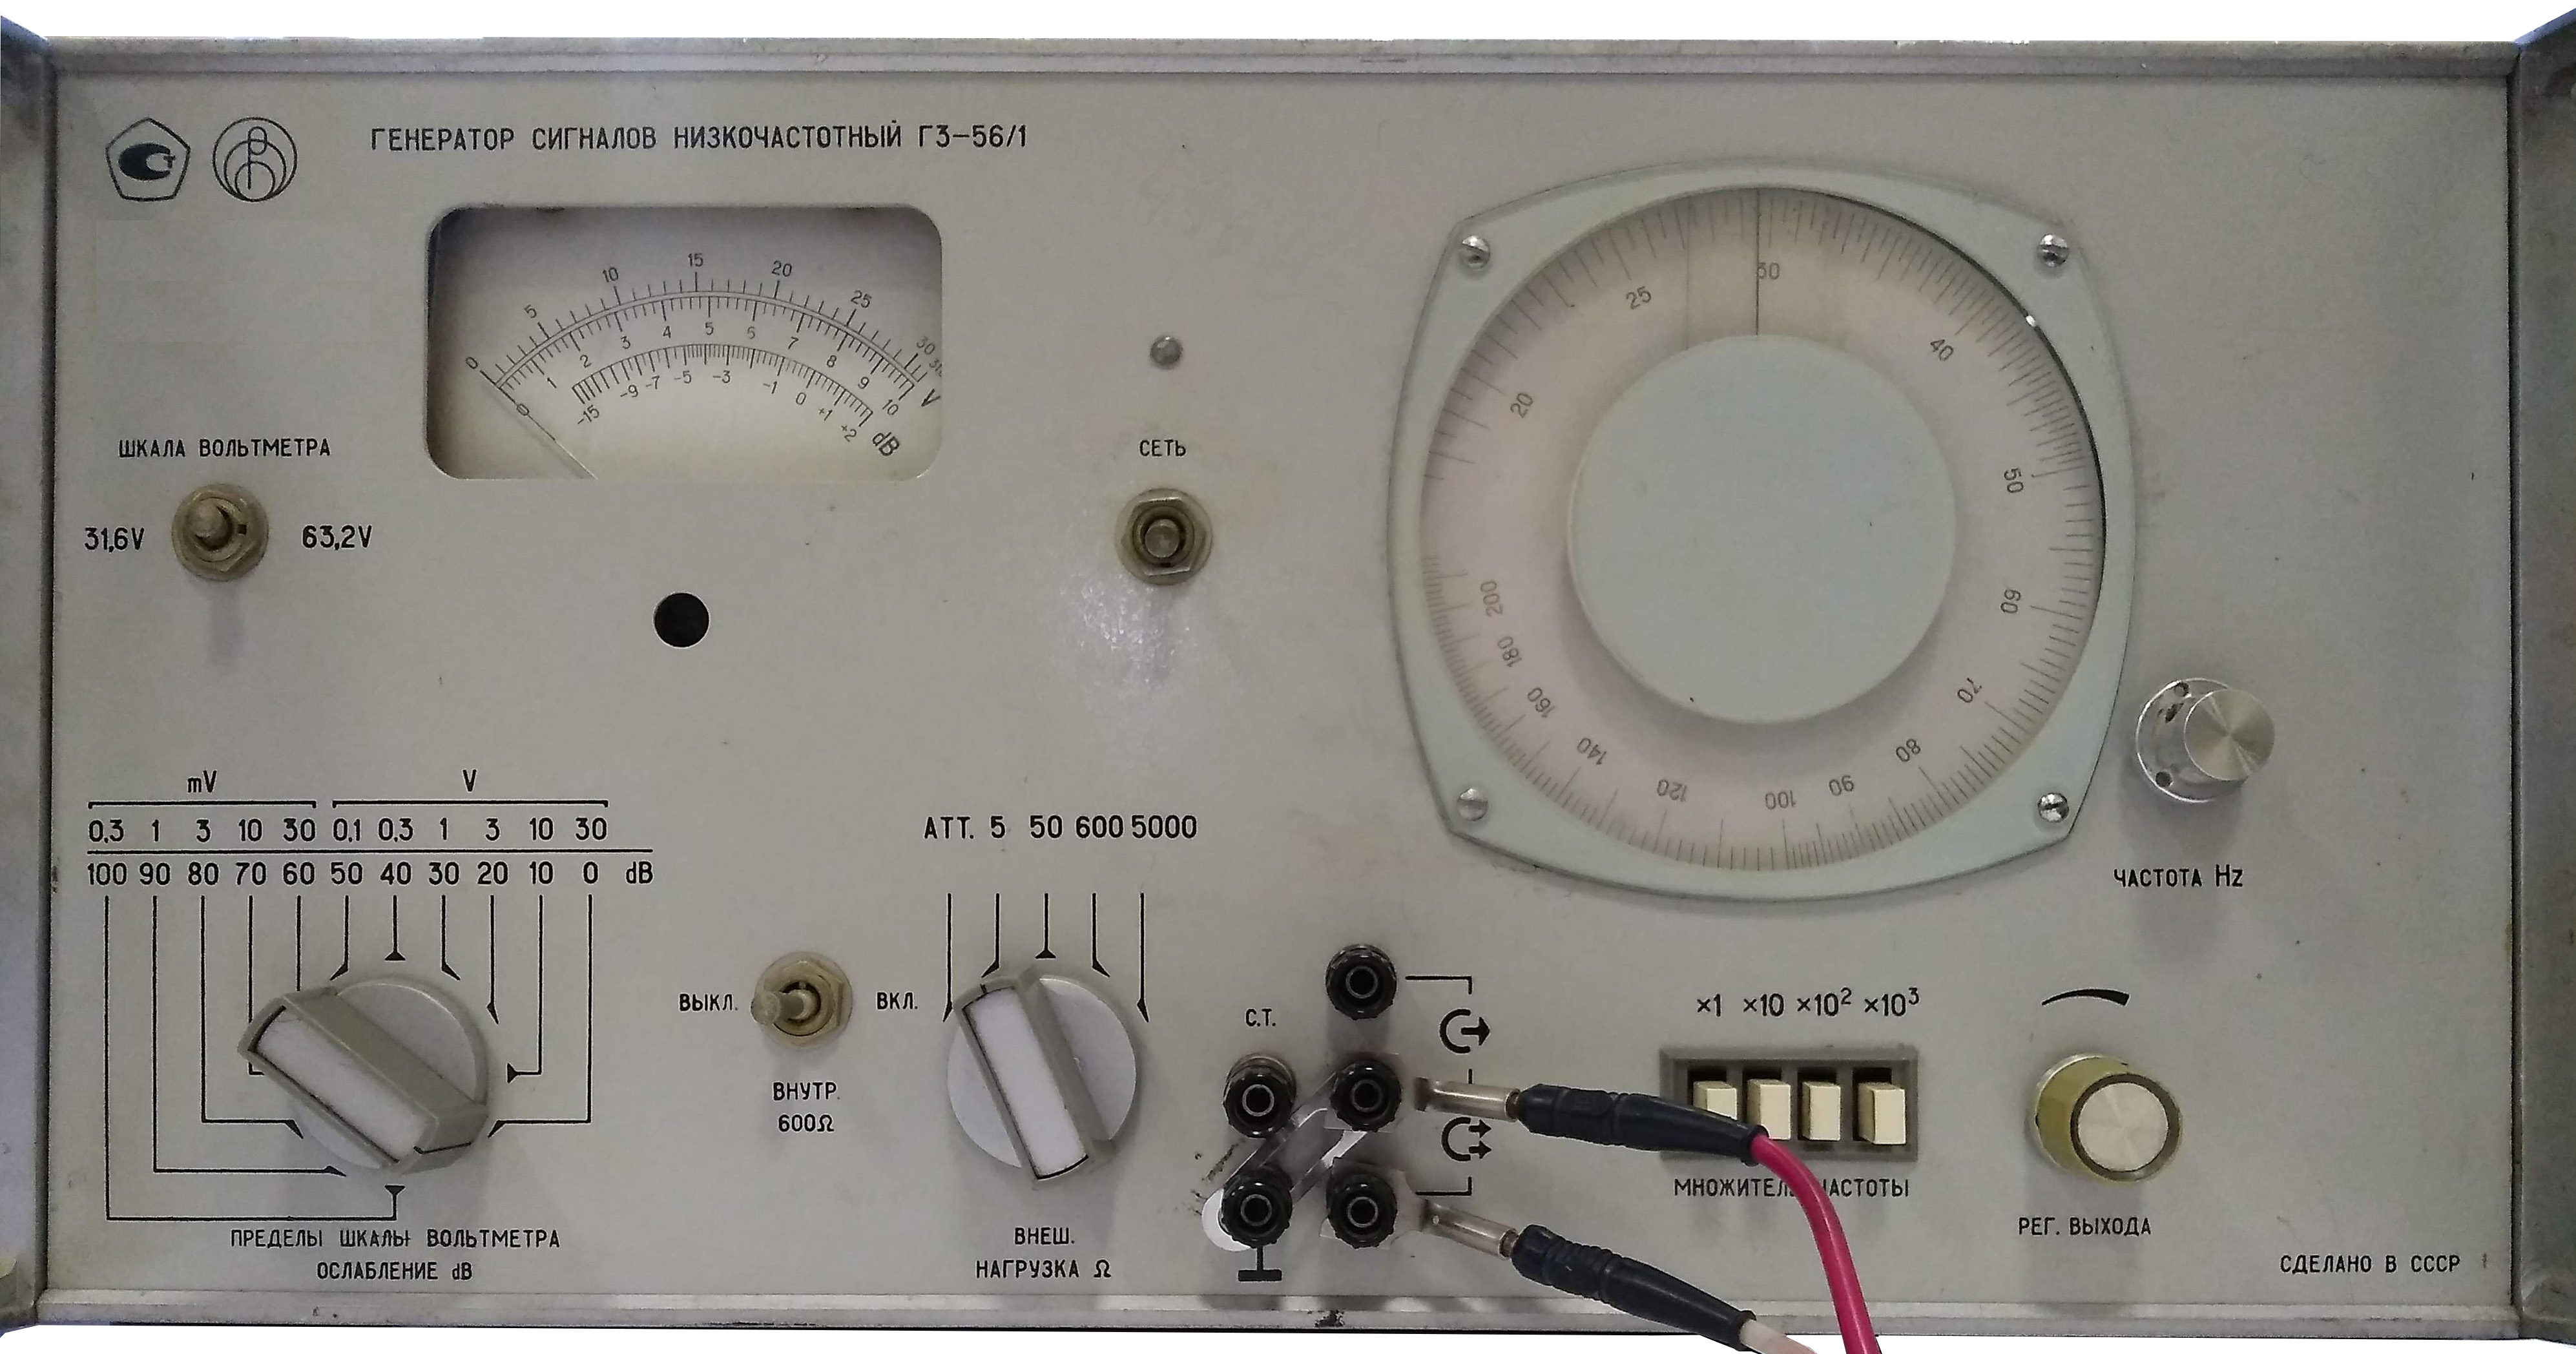
\includegraphics[width=12cm]{\currfiledir/GZ56}};
    \node[small dot,pin={[pin distance=2.5cm]90:{\ref{btn:powerGZ56}}}] at (-0.6,0.6) {};
    \node[small dot,pin={[pin distance=1.8cm]0:{\ref{btn:fHz}}}] at (4.4,-0.2)  {};
    \node[small dot,pin={[pin distance=1.2cm]-90:{\ref{btn:fMulyiply}}}] at (2.5,-2)  {};
    \node[small dot,pin={[pin distance=2.3cm]90:{\ref{scale:freq}}}] at (2.2,0.8)  {};
    \node[small dot,pin={[pin distance=1.05 cm]-90:{\ref{btn:regexit}}}] at (3.9,-2.1)  {};
    \node[small dot,pin={[pin distance=1.2cm]180:{\ref{btn:Vscale}}}] at  (-5,0.7) {};
    \node[small dot,pin={[pin distance=1.1cm]-90:{\ref{btn:VscaleLim}}}] at  (-4.2,-2) {};
    \node[small dot,pin={[pin distance=1.1cm]90:{\ref{scale:Vscale}}}] at (-2.8,2) {};
    \node[small dot,pin={[pin distance=1.2cm]-90:{\ref{btn:ExtR}}}] at (-1.2,-2) {};
    \node[small dot,pin={[pin distance=1.6cm]-90:{\ref{btn:IntR}}}] at (-2.3,-1.5) {};
%    \draw[red] (-6,-3) to [grid with coordinates] (6,3);
\end{tikzpicture}
\caption{Елементи керування генератором ГЗ-56/1}
\label{fig:gz56}
\end{figure}

На рис.~\ref{fig:gz56} показані основні органи керування генератором: 

\begin{enumerate}
    \item \label{btn:powerGZ56} ручка вмикання/вимикання живлення;
    \item \label{btn:fHz} Ручка \circled{\ref{btn:fHz}} \tcbox{\sc{ЧАСТОТА Hz}} для плавної установки частоти в межах кожного піддіапазону;
    \item \label{btn:fMulyiply} перемикачі \circled{\ref{btn:fMulyiply}} \tcbox{\sc{МНОЖИТЕЛЬ ЧАСТОТЫ}} для перемикання піддіапазонів (в залежності від необхідної частоти натиснута одна з кнопок множника);
    \item \label{scale:freq} циферблат шкали частотометра;
    \item \label{btn:regexit} ручка  \circled{\ref{btn:regexit}} \tcbox{\sc{РЕГ. ВЫХОД}} для плавного регулювання вихідної напруги на несиметричному і додатковому симетричному виходах;
    \item \label{scale:Vscale} вольтметр для контролю вихідної напруги;
    \item \label{btn:Vscale}тумблер \circled{\ref{btn:Vscale}} \tcbox{\sc{ШКАЛА ВОЛЬТМЕТРА}} для перемикання шкал стрілочного приладу;
     \item \label{btn:VscaleLim} ручка \tcbox{\sc{ПРЕДЕЛЫ ШКАЛЫ ВОЛЬТМЕТРА / ОСЛАБЛЕНИЕ dB}} для введення загасання від 0 до 100 дБ;;
    \item \label{btn:ExtR} перемикач \circled{\ref{btn:ExtR}} \tcbox{\sc{ВНЕШ. НАГРУЗКА $\Omega$ / АТТ}} для перемикання обмоток узгоджувальних трансформаторів в залежності від зовнішнього навантаження; в положенні перемикача \tcbox{\sc{АТТ}} сигнал з вихідного підсилювача приходить на вихідні клеми генератора через атенюатор. 
    \item \label{btn:IntR}за допомогою перемикача \circled{\ref{btn:IntR}} \tcbox{\sc{ВНУТР. 600 $\Omega$ }} на виході атенюатора включається навантаження $600$~Ом;
    \item клема \sc{С.Т.} середня точка узгоджувальних трансформаторів, яка за допомогою спеціальної шини може з'єднуватися з клемою $\perp$.
    \item клема \tikz[baseline=-0.3em]{\draw[thick] (90:0.5em) arc (90:270:0.5em); \draw[-latex,thick] (0,0) -- ++(0.75em,0);}  для роботи на несиметричному виході;
    \item  клеми \tikz[baseline=-0.3em]{\draw[thick] (90:0.5em) arc (90:270:0.5em); \draw[-latex,thick] (0,0.1) -- ++(0.75em,0);\draw[-latex,thick] (0,-0.1) -- ++(0.75em,0);}  для роботи на симетричному виході;
\end{enumerate}

\subsection*{Вольтметр \href{https://www.youtube.com/watch?v=qBjsfKW9BbE}{\sc{В7-16А}}}

\begin{figure}[h!]
\centering
\begin{tikzpicture}[every pin/.style={minimum size = 5pt, pin edge={red, thick}, draw, fill=gray!5, red, circle, font=\scriptsize},
    small dot/.style={fill=black,circle,scale=0.3}]
    \node at (0,0){ 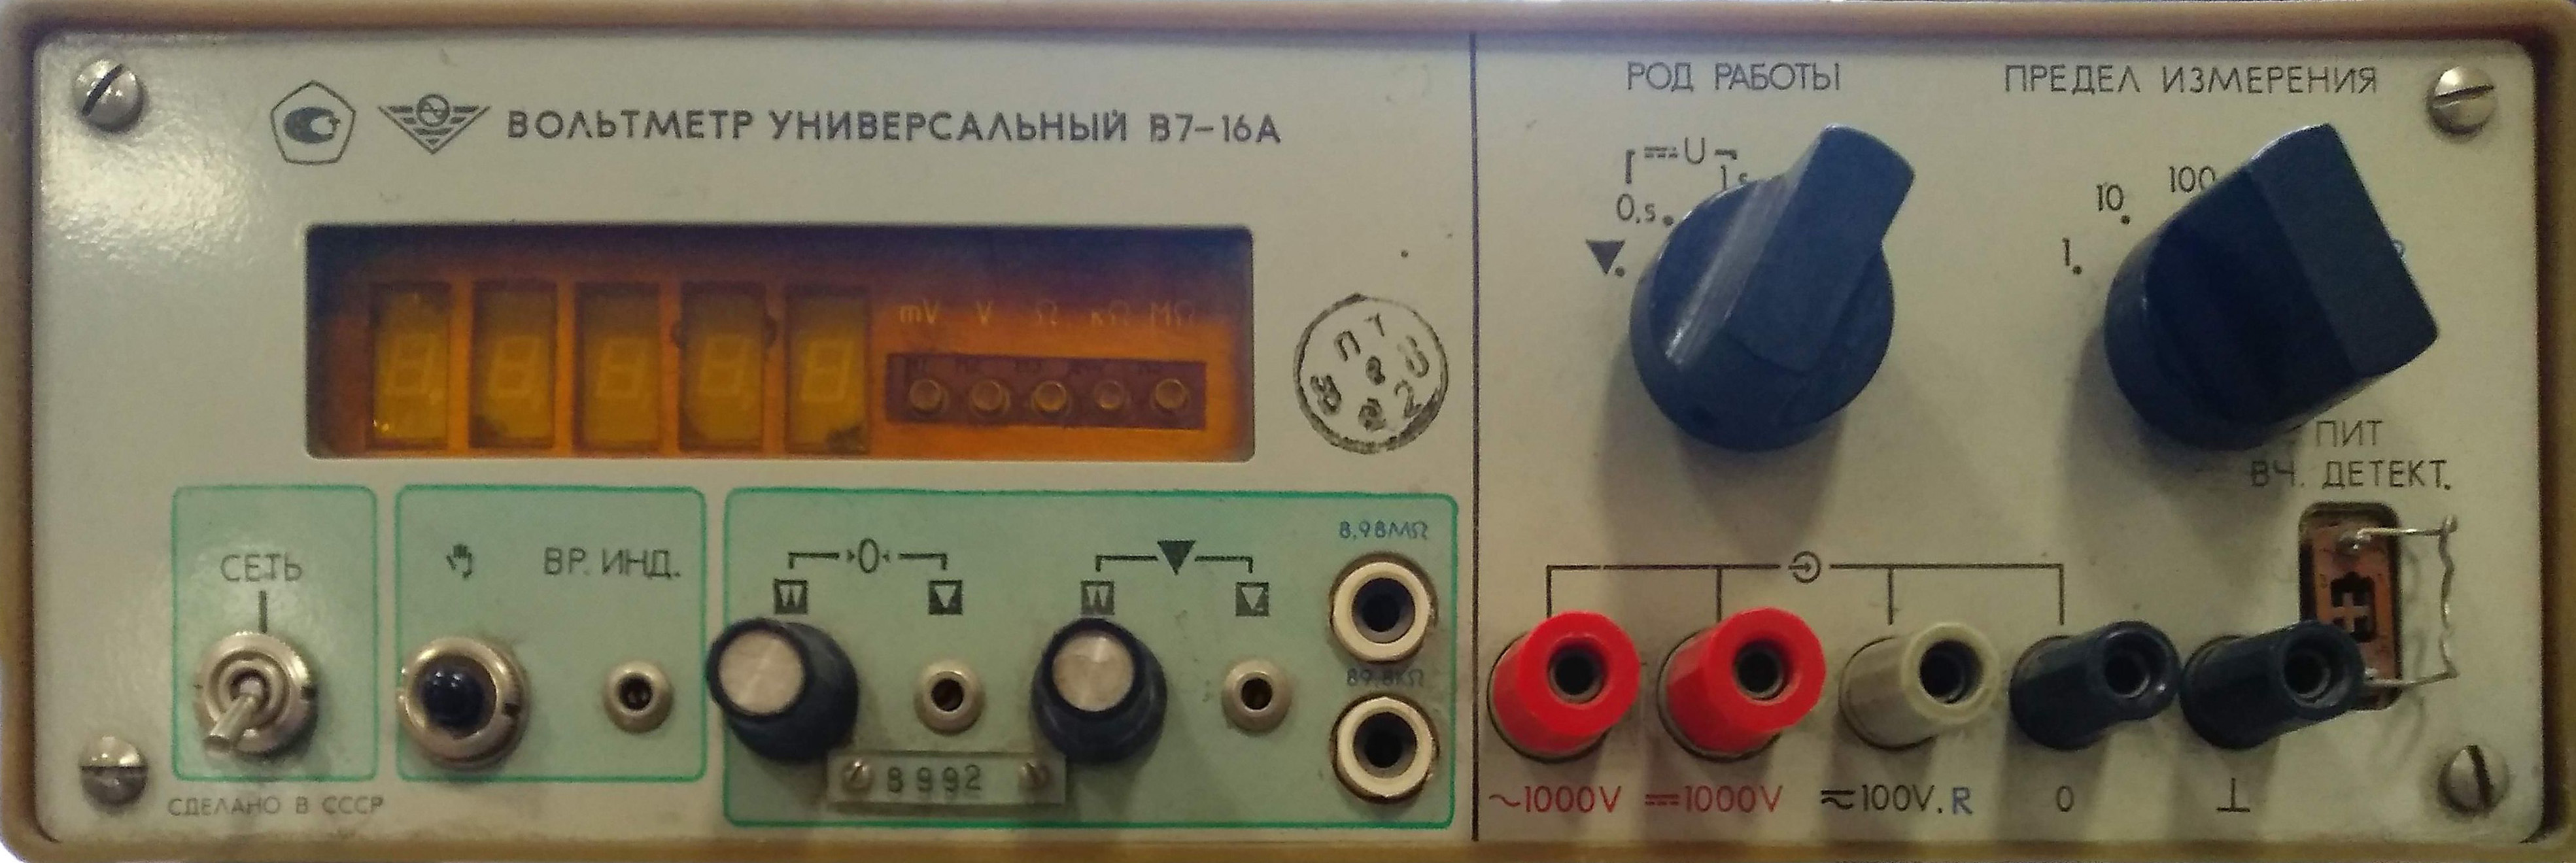
\includegraphics[width=12cm]{\currfiledir/V716A}};
    \node[small dot,pin={[pin distance=0.8cm]-90:{\ref{btn:powerV716A}}}] at (-4.9,-1.3) {};
    \node[small dot,pin={[pin distance=1cm]-90:{\ref{btn:O}}}] at (-2.5,-1.1)  {};
    \node[small dot,pin={[pin distance=1cm]-90:{\ref{btn:Tri}}}] at (-0.9,-1.1)  {};
    \node[small dot,pin={[pin distance=1.5cm]90:{\ref{btn:Rod}}}] at (2.4,0.6)  {};
    \node[small dot,pin={[pin distance=1.5cm]90:{\ref{btn:Limit}}}] at (5,0.6)  {};
    \node[small dot,pin={[pin distance=1cm]-90:{\ref{pin:AltCur}}}] at (1.35,-1.15)  {};
    \node[small dot,pin={[pin distance=1cm]-90:{\ref{pin:SteadCur}}}] at (2.25,-1.15)  {};
    \node[small dot,pin={[pin distance=1cm]-90:{\ref{pin:Ohm}}}] at (3.1,-1.15)  {};
    \node[small dot,pin={[pin distance=1cm]-90:{\ref{pin:O}}}] at (3.9,-1.15)  {};
    \node[small dot,pin={[pin distance=1cm]-90:{\ref{pin:ground}}}] at (4.8,-1.15)  {};
\end{tikzpicture}
\caption{Елементи керування вольтметром \sc{В7-16А}}
\label{fig:V716A}
\end{figure}

На рис.~\ref{fig:V716A} показані основні органи керування вольтметром: 

\begin{enumerate}
    \item \label{btn:powerV716A} вмикач живлення;
    \item \label{btn:O} ручка потенціометру корекції нуля;
    \item \label{btn:Tri} ручка потенціометру калібрування;
    \item \label{btn:Rod} перемикач роду роботи для вибору режимів вимірювання напруг до $100$~В та активного опору;
    \item \label{btn:Limit} перемикач меж вимірювання при вимірюваннях напруг до $100$~В та активного опору;
     \item \label{pin:O} загальна клема при вимірюваннях;
     \item \label{pin:AltCur} клема для вимірювання змінної напруги від $100$ до $1000$~В;
     \item \label{pin:SteadCur} клема для вимірювання постійної напруги від $100$ до $1000$~В;
     \item \label{pin:Ohm} клема для вимірювання змінної, постійної напруги до $100$~В та опору в залежності від положення ручки \tcbox{\sc{РОД РАБОТЫ}} ;
     \item \label{pin:ground} клема заземлення вольтметра
\end{enumerate}

\section{Методика дослідження}

\subsection{Реальні елементи електричного кола. Схеми заміщення}

В реальному контурі конденсатор і котушка окрім ємнісного $X_C$ та індуктивного опорів $X_L$ також мають і активні опори $R_C$ та $R_L$. Активний опір конденсатора $R_C$ зумовлений струмами провідності в прошарку діелектрика, а котушки $R_L$~--- матеріалом дротів намотки. Для урахування цього,  схеми які містять реальні елементи можна замінити на еквівалентні схеми, в яких позначення конденсатора і котушки представляють собою ідеальні елементи, а їхні активні опори зображують окремо у вигляді резисторів. Однак, таке представлення не є однозначним і залежить від частот, на яких працює контур. Так, наприклад, за частот при яких $X_C \ll R_C$ реальний конденсатор зручно заміщати ланцюжком вигляду, зображеному на рис.~\ref{pic:equiv_capacitor}. Котушка індуктивності ж за частот, при яких $X_L \gg R_L$ заміщається ланцюжком вигляду~\ref{pic:equiv_inductor}. Для досліджуваного в лабораторній роботі діапазону частот ці два випадки задовольняються одночасно, оскільки, активний опір конденсатора дуже великий ($\approx 10^2$~МОм), а у котушки дуже малий $0.8$~Ом. Окрім того, реальний генератор має свій внутрішній опір $R_i$ і тому його також можна зобразити у вигляді схеми заміщення~\ref{pic:equiv_ac_generator}.
  
%Для послідовного і паралельного контурів такі схеми можуть виглядати по різному. 

%=========================================================
\begin{figure}[h!]\centering
	% !TeX program = lualatex
% !TeX encoding = utf8
% !TeX spellcheck = uk_UA
% !TeX root =../LabWork.tex

	%---------------------------------------------------------
	\begin{minipage}[t]{0.3\linewidth}
		\centering
		\begin{tikzpicture}[thick, every circuit symbol/.style={thick}]
			\draw (0,0) node[contact] {} to [capacitor={info={$C$}}] ++(4,0) node[contact] {} (1,0) -- ++(0,-1) to [resistor={info={$R_C$}, color=red}] ++(2,0) -- ++ (0,1);
		\end{tikzpicture}
		\caption{Схема заміщення реального конденсатора}
		\label{pic:equiv_capacitor}
	\end{minipage}
	\quad%---------------------------------------------------------
	\begin{minipage}[t]{0.3\linewidth}
		\centering
		\begin{tikzpicture}[thick, every circuit symbol/.style={thick}]
			\draw (0,0) node[contact] {} to [resistor={info={$R_L$}, color=red}] ++(2,0) to [inductor={info={$L$}}] ++(2,0) node[contact] {};
			\path (0,0) -- ++(0,-1.05);
		\end{tikzpicture}
		\caption{Схема заміщення реальної котушки}
		\label{pic:equiv_inductor}
	\end{minipage}
	\quad%---------------------------------------------------------
	\begin{minipage}[t]{0.3\linewidth}
		\centering
		\begin{tikzpicture}[thick, every circuit symbol/.style={thick}]
			\draw (0,0) node[contact] {} to [resistor={info={$R_i$}, color=red}] ++(2,0) to [ac source={info={$\mathcal{E}$}}] ++(2,0) node[contact] {};
			\path (0,0) -- ++(0,-1.05);
		\end{tikzpicture}
		\caption{Схема заміщення реального генератора}
		\label{pic:equiv_ac_generator}
	\end{minipage}
	%---------------------------------------------------------
\end{figure}
%=========================================================

%\begin{wrapfigure}{L}{0.45\linewidth}
%	\centering
%	\begin{tikzpicture}[thick, every circuit symbol/.style={thick}]
%		\draw (0,-2) coordinate (START) to [resistor={info={$R_i$}, color=red}] ++(0,2) to [ac source={rotate=-90,info={left:$\mathcal{E}$}}] (0,2) to [resistor={info={$R_I$}}] coordinate (V1) ++(4,0) to [inductor={info={$L$}}] ++(0,-4/3) to [resistor={info={$R_{L}$}, color=red}] ++(0,-4/3) to [capacitor={info={$C$}}] ++(0,-4/3)  -- (START);
%		\draw ([xshift=-0.75cm]V1) node [contact] {} -- ++(0,1) to [voltmeter] ++(1.5,0) -- ++(0,-1)  node [contact] {};
%	\end{tikzpicture}
%	\caption{Послідовне з'єднання елементів}
%	\label{pic:equiv_serial_circuit}
%\end{wrapfigure}
%З урахуванням схем заміщення, еквівалентна схема при послідовного кола зображується у вигляді, поданому на рис.~\ref{pic:equiv_serial_circuit}. В даному випадку, активний опір конденсатора  настільки великий, що його врахування практично не дає ніякого вкладу в дослідження резонансних явищ, а тому він не позначений на схемі.



\subsection{Опис методики дослідження}


На коливальний контур подають синусоїдальну зовнішню напругу з контрольованою частотою $\omega = 2\pi \nu$, вимірюють залежність струму від частоти.

У випадку послідовного з'єднання конденсатора і котушки індуктивності на резонансній частоті $\omega_0$ повинні спостерігатися максимум амплітуди струму (напруги на резисторі $R_I$). При паралельному з'єднанні конденсатора і котушки резонанс в контурі виявляють по мінімальній напрузі на резисторі $R_I$, або по максимальній напрузі на конденсаторі і котушці.


Для дослідження явища резонансу використовують електричні кола, наведені на рис.~\ref{pic:serial_circuit} та \ref{pic:paralel_circuit}. Коло з послідовно з'єднаними елементами $L$ і $C$ (рис.~\ref{pic:serial_circuit}) призначене для вивчення резонансу напруг, а коло з паралельним з'єднанням  $L$ і $C$ (рис.~\ref{pic:paralel_circuit}) --- для резонансу струмів.  Оскільки активний опір конденсатора  настільки великий, що його врахування практично не дає ніякого вкладу в дослідження резонансних явищ, а тому він не позначений на схемах.

У випадку послідовного кола, для визначення струму, вимірюють напругу на резисторі $R_I$ за допомогою вольтметру універсального \sc{В7-16А}, для вимірювань напруги на $LC$-ланцюжку використовується осцилограф \sc{C1-83}.

Завдяки наявності активного опору котушки, напруга на $LC$-ланцюжку при резонансі~\eqref{ULC} не дорівнюватиме нулю:
\[
	U_{0_{LC}} = U_{0_L} - U_{0_C} = I_0 R_L \approx 0,
\]
в чому можна переконатись, під'єднавши осцилограф при резонансі до цієї ділянки кола. Іншими словами, імпеданс цього ланцюжка стає найменшим і дорівнює його активному опору $R_L$ (який має порівняно невелику величину).

%=========================================================
\begin{figure}[!h]\centering
	%---------------------------------------------------------
	\begin{minipage}[t]{0.45\linewidth}
		\centering
		\begin{tikzpicture}[thick, every circuit symbol/.style={thick}]
			%			\draw[blue, fill=blue!20] (1,1.5) rectangle ++(2,2);
			\draw[red, fill=red!20] (-0.7,-1.6) rectangle ++(1.2,3.1);
			\draw (0,-2) coordinate (START) to [resistor={info={$R_i$}, color=red}] ++(0,2) to [ac source={rotate=-90,info={left:$\mathcal{E}$}}] ++(0,2) to [resistor={info={$R_I$}}] coordinate (V1) ++(4,0) to [resistor={info={$R_{L}$}, color=red}] ++(0,-4/3) to [inductor={info={$L$}}] ++(0,-4/3) to [capacitor={info={$C$}}] ++(0,-4/3)  -- (START)
			;
			\draw ([xshift=-0.75cm]V1) node [contact] {} -- ++(0,1) to [voltmeter] ++(1.5,0) -- ++(0,-1)  node [contact] {};
		\end{tikzpicture}
		\caption{Послідовне з'єднання елементів}
		\label{pic:serial_circuit}
	\end{minipage}
	\quad%---------------------------------------------------------
	\begin{minipage}[t]{0.47\linewidth}
		\centering
		\begin{tikzpicture}[thick, every circuit symbol/.style={thick}]
			\draw[red, fill=red!20] (-0.7,-1.6) rectangle ++(1.2,3.1);
			\draw (0,-2) coordinate (START) to [resistor={info={$R_i$}, color=red}] ++(0,2) to [ac source={rotate=-90,info={left:$\mathcal{E}$}}] (0,2) to [resistor={info={$R_I$}}] ++(2,0)  coordinate (V1) -- ++(2,0) -- ++(0,-3/4) node [contact] {}  coordinate (C)

			(C) -- ++(1,0) to [resistor={info={$R_L$}, color = red}]  ++(0,-5/4) to [inductor={info={$L$}}] ++(0,-5/4)   --  ++(-1,0) coordinate (B) node [contact] {}
			(C) -- ++(-1,0) to [capacitor={info={$C$}}] ++(0,-10/4)  -- ++(1,0)
			(B) -- ++(0,-3/4)  -- (START);
			\draw (C) to [resistor={info={$R$}}] (B);
			\draw[] (V1) node [contact] {} to[voltmeter] ++(0,-4) node [contact] {};
			\draw (V1) node [contact] {} -- ++(0,1) to [voltmeter] ++(-2,0) -- ++(0,-1)  node [contact] {};
		\end{tikzpicture}
		\caption{Паралельне з'єднання елементів}
		\label{pic:paralel_circuit}
	\end{minipage}
	%---------------------------------------------------------
\end{figure}

%=========================================================
\section{Підготовка до рботи}

\subsection*{Початкове положення органів до включення в мережу}

\subsubsection*{Генератор \sc{Г3-56/1}}

\begin{enumerate}
	\item Перемикач \circled{\ref{btn:VscaleLim}}  \tcbox{\sc{ОСЛАБЛЕНИЕ dB}} --- в положенні \tcbox{\sc{0}} ;
	\item тумблер \circled{\ref{btn:IntR}}  \tcbox{\sc{ВНУТР. 600 Ω}} --- в положенні \tcbox{\sc{ВКЛ.}};
	\item перемикач \circled{\ref{btn:ExtR}}  \tcbox{\sc{ВНЕШ. НАГРУЗКА Ω}} --- в положенні \tcbox{\sc{5}};
	\item увімкнена одна з кнопок перемикача \circled{\ref{btn:fMulyiply}}  \tcbox{\sc{МНОЖИ­ТЕЛЬ ЧАСТОТЫ}};
	\item ручка \circled{\ref{btn:regexit}}  \tcbox{\sc{РЕГ. ВЫХОДА}} знаходиться в середньому положенні;
	\item ручки \circled{\ref{btn:fHz}}  \tcbox{\sc{ЧАСТОТА Hz}} --- в довільному положенні;
	\item тумблер \circled{\ref{btn:Vscale}}  \tcbox{\sc{ШКАЛА ВОЛЬТМЕТРА}} --- в положенні \sc{63,2 V}.
\end{enumerate}

\subsubsection*{Вольтметр {\sc{В7-16А}} та осцилограф {\sc{C1-83}}}

\begin{enumerate}
	\item На вольтметрі \sc{В7-16А} встановіть ручку \circled{\ref{btn:Limit}} \tcbox{\sc{ПРЕДЕЛ ИЗМЕРЕНИЯ}} в положення \tcbox{\sc{10}}, ручку \circled{\ref{btn:Rod}} \tcbox{\sc{РОД РАБОТЫ}}  в положення \tcbox{\sc{$\sim$ U}}. Для підключення вольтметра використовуйте чорну клему входу  \circled{\ref{pin:O}} \tcbox{\sc{0}} та білу клему  \circled{\ref{pin:Ohm}} \tcbox{\sc{$\simeq$ 100 V}}. Також врахуйте, що вхідний опір вольтметра в режимі вимірювання змінного струму становить всього $1$~МОм, тому не рекомендується ним вимірювати напругу на паралельному $RLC$~колі, натомість використовуйте осцилограф.
	\item На осцилографі {\sc{C1-83}} встановіть ручку \tcbox{\sc{V/ДЕЛ}} на \tcbox{\sc{Канал I}} в положення \tcbox{\sc{5}}.
\end{enumerate}

\subsection*{Положення органів після включення приладів в мережу}

\begin{enumerate}
	\item Ручкою \circled{\ref{btn:regexit}} \tcbox{\sc{РЕГ. ВЫХОДА}} на генераторі \tcbox{\sc{ГЗ-56/1}} встановіть максимальну напругу генератора (дивіться на шкалу вольтметра генератора~\circled{\ref{scale:Vscale}}).
\end{enumerate}

\section{Завдання}

\begin{enumerate}
	\item Визначте внутрішній активний опір генератора $R_i$.
	\item Зберіть електричне коло за схемами
	      \begin{enumerate}[label=\alph*)]
		      \item послідовного з'єднання~\ref{pic:serial_circuit} ($R_I = 10$~Ом; $50$~Ом, $C = 1.2$~мкФ);
		      \item паралельного з'єднання~\ref{pic:paralel_circuit} ($R_I = 10$~Ом, $R = 1$~кОм; $2.2$~кОм та $C = 1.2$~мкФ). В якості вольтметра на резисторі $R_I$ використовуйте прилад \sc{В7-16А}, в якості вольтметра для $RLC$~ланцюжка -- осцилограф.
	      \end{enumerate}
	      {\small\itshape На схемах в червоному прямокутнику показано генератор змінної напруги зі своїм внутрішнім опором $R_i$, в синьому прямокутнику показано під'єднання вольтметру до резистора відомого опору для вимірювання сили струму в колі.}
	\item Переконайтесь за допомогою осцилографа, що \emph{при резонансі} у випадку
	      \begin{enumerate}[label=\alph*)]
		      \item послідовного контуру~\ref{pic:serial_circuit}  напруга на $LC$-ділянці досягає мінімального значення;
		      \item паралельного контуру~\ref{pic:paralel_circuit} струм в колі досягає мінімального значення (для цього заміряйте напругу на резисторі $R_I$).
	      \end{enumerate}
	\item Зніміть амплітудно-частотні характеристики в досліджуваному колі. Приклад АЧХ для послідовного кола (рис.~\ref{plt:AchKh_serial}).
	\item Визначте добротність електричного кола та резонансну частоту.
	\item Розрахуйте загальний опір втрат.
	\item Розрахуйте теоретично добротність електричного кола та резонансну частоту враховуючи отримане значення опору втрат, та порівняйте їх з експериментальними значеннями.
	\item Оцініть похибки вимірювання.
\end{enumerate}

\begin{figure}[!h]\centering
    % !TeX program = lualatex
% !TeX encoding = utf8
% !TeX spellcheck = uk_UA
% !TeX root =../LabWork.tex



%---------------------------------------------------------
\begin{center}
	\begin{tikzpicture}[
			declare function={
					L  = 2e-3;
					C  = 1.2e-6;
					R  = 10;
					RL  = 0.8;
					Ri  = 5;
					Rtot = R + RL + Ri;
					U  = 10;
					omegares  = 1/sqrt(L*C);
					nures  = omegares/(2*pi);
					Q  = sqrt(L/C)/Rtot;
					Imax  = U/Rtot;
					D1 =  (1/(4*pi*L))*(sqrt( (Rtot^2+4*L/C)) - Rtot);
					D2 = (1/(4*pi*L))*(sqrt( (Rtot^2*C+4*L)/C) + Rtot);
					I(\x) = Rtot/sqrt(Rtot^2 + ((2*pi*\x)*L-1/(C*(2*pi*\x)))^2);
					F2(\x) = sqrt(Rtot^2/(pi^2*\x^2*L^2) + sqrt(((\x^2 - 1)*Rtot^2*(\x^2*C*Rtot^2 - 4*\x^2*L - C*Rtot^2))/(\x^4*C))/(pi^2*L^2) + 2/(pi^2*C*L) - Rtot^2/(pi^2*L^2))/(2*sqrt(2));
					F1(\x) = sqrt(Rtot^2/(pi^2*\x^2*L^2) - sqrt(((\x^2 - 1)*Rtot^2*(\x^2*C*Rtot^2 - 4*\x^2*L - C*Rtot^2))/(\x^4*C))/(pi^2*L^2) + 2/(pi^2*C*L) - Rtot^2/(pi^2*L^2))/(2*sqrt(2));
				},
		]


		\begin{axis}[
				% === Налаштування сітки ===
				grid = both,
				major grid style={line width=.6pt,draw=brown!60},
				minor tick num = 9,
				minor grid style = {line width=.1pt,draw=brown!20},
				% === Налаштування положення координатних осей ===
				axis lines = middle,
				axis line style={-stealth},
				% === Підпис координатних осей ===
				%				xticklabels={},
				xlabel={$\nu$, Hz},
				ylabel={$\frac{I_{0}}{I_{\max}}$},
				% === Положення підпису координатних осей ===
				ylabel style={above right},
				every tick/.style={black},
				extra tick style={% changes for all extra ticks
						tick align=outside,
						major grid style={dashed,draw=black}
					},
			    extra x tick style={
			      red,
			      major tick style={
			        gray,
			      },
			      tick label style={
					yshift=10mm,
			        /pgf/number format/.cd, fixed, fixed zerofill,
			        precision=2,
			      }
			    },
				extra y tick style={% changes for extra y ticks
						tick label style={yshift=2mm},
					},
				extra x ticks={F1(1/sqrt(2)), nures, F2(1/sqrt(2)},
				extra x tick labels={
					\pgfmathprintnumberFE[custom exponent=0]{F1(1/sqrt(2))/100},
					\pgfmathprintnumberFE[custom exponent=0]{nures/100},
					\pgfmathprintnumberFE[custom exponent=0]{F2(1/sqrt(2))/100},
					},
				extra y ticks={1/sqrt(2)},
				extra y tick labels={$1/\sqrt{2}$},
				scaled x ticks=base 10:-2,
				% === Вибір підписів шкали для відображення ===
				xtick = {},
				ytick = {},
				% === Налаштування мінімальних та максимальних значень координат ===
				xmin = 15e2,
				xmax =  65e2,
				ymin = 0.25,
				ymax =  1,
				% === Налаштування розміру графіка ===
				width=1\linewidth,
				height=0.85\textheight,
			]
			\addplot [ultra thick,samples = 500, green!50!black, thick, domain=0.51*nures:1.85*nures, name path global=ResCurve]  {I(x)};


			\pgfplotsinvokeforeach{0.3,0.4,...,0.9}
			{
				\addplot[color=blue,mark=*, only marks, point meta=x, nodes near coords={\pgfmathprintnumberFE[custom exponent=0, precision=1]{\pgfplotspointmeta/100}}, every node near coord/.append style={anchor=west}] coordinates { (F1(#1),#1) (F2(#1),#1) };
			}
			\addplot[color=red,mark=*, only marks, point meta=x, nodes near coords={\pgfmathprintnumberFE[custom exponent=0, precision=1]{\pgfplotspointmeta/100}}, every node near coord/.append style={anchor=south}] coordinates {(F2(1),1)};


			%			\fill [white, draw=green!50!black, name intersections={of=ResCurve and line}] (intersection-1) circle (0.05cm) (intersection-2) circle (0.05cm);
			\node[anchor = north east, text width=6cm] at (current axis.north east) {
				\begin{tornpage}
					$C = \pgfmathprintnumberFE[custom exponent=-6,precision=1]{C}$~Ф,\\
					$L = \pgfmathprintnumberFE[custom exponent=-3,precision=0]{L}$~Гн,\\
					$R_L = \pgfmathprintnumberFE[custom exponent=0,precision=2]{RL}$~Ом,\\
					$R_i = \pgfmathprintnumberFE[custom exponent=0,precision=2]{Ri}$~Ом,\\
					$R_I = \pgfmathprintnumberFE[custom exponent=0,precision=2]{R}$~Ом,\\
					\hrulefill\\
					\medskip%
					$Q^{\mathrm{theor}} = \dfrac{1}{R}\sqrt{\dfrac{L}{C}} = \pgfmathprintnumberFE[custom exponent=0,precision=2]{Q}$\\
					\hrulefill\\
					\smallskip%
					$\nu_0 = \pgfmathprintnumberFE[custom exponent=2,precision=1]{nures}$~Hz \\
					$2\Delta\nu = \pgfmathprintnumberFE[custom exponent=2,precision=1]{D2-D1}$~Hz\\
					\hrulefill\\
					\smallskip%
					$Q^{\mathrm{exp}} = \dfrac{\nu_0}{2\Delta\nu} = \pgfmathprintnumberFE[custom exponent=0,precision=2]{nures/(D2-D1)}$
				\end{tornpage}
			};
		\end{axis}
	\end{tikzpicture}
\end{center}

    \caption{Експериментальна АЧХ для послідовного кола}
    \label{plt:AchKh_serial}
\end{figure}

\section*{Контрольні запитання}

\begin{enumerate}
	\item Які струм називається квазістаціонарним? Що розуміють під терміном <<змінний струм>>?
	\item Поясніть метод комплексних амплітуд та сформулюйте на їх основі правила Кірхгофа для кіл змінного струму.
	\item Що таке імпеданс?
	\item Що таке активний та реактивний опори?
	\item Що таке добротність електричного кола?
	\item Опишіть явища резонансу напруг та струмів в колах змінного струму.
\end{enumerate}

